\chapter{栈和队列}

栈(stack)只能在表的一端插入和删除,先进后出(LIFO, Last In, First Out)。

队列(queue)只能在表的一端(队尾rear)插入,另一端(队头front)删除,先进先出(FIFO, First In, First Out)。

\section{栈} %%%%%%%%%%%%%%%%%%%%%%%%%%%%%%

\subsection{栈的C语言实现}
C++可以直接使用\fn{std::stack}。

\begin{Codex}[label=stack.c]
/**
 * @file stack.c
 * @brief 栈,顺序存储.
 * @author soulmachine@gmail.com
 */
#include <stdlib.h>  /* for malloc() */
#include <string.h>  /* for memcpy() */

typedef int stack_elem_t; // 元素的类型

/**
 * @struct
 * @brief 栈的结构体
 */
typedef struct stack_t {
    int     size;  /** 实际元素个数 */
    int     capacity; /** 容量,以元素为单位 */
    stack_elem_t  *elems;   /** 栈的数组 */
}stack_t;

/**
 * @brief 创建栈.
 * @param[in] capacity 初始容量
 * @return 栈对象的指针
 */
stack_t* stack_create(const int capacity) {
    stack_t *s = (stack_t*)malloc(sizeof(stack_t));
    s->size = 0;
    s->capacity = capacity;
    s->elems = (stack_elem_t*)malloc(capacity * sizeof(stack_elem_t));
    return s;
}

/**
 * @brief 销毁栈.
 * @param[inout] s 栈对象的指针
 * @return 无
 */
void stack_destroy(stack_t *s) {
    free(s->elems);
    free(s);
}

/**
 * @brief 判断栈是否为空.
 * @param[in] s 栈对象的指针
 * @return 是空,返回 1,否则返回 0
 */
int stack_empty(const stack_t *s) {
    return s->size == 0;
}

/**
 * @brief 获取元素个数.
 * @param[in] s 栈对象的指针
 * @return 元素个数
 */
int stack_size(const stack_t *s) {
    return s->size;
}

/**
 * @brief 进栈.
 * @param[in] s 栈对象的指针
 * @param[in] x 要进栈的元素
 * @return 无
 */
void stack_push(stack_t *s, const stack_elem_t x)
{
    if(s->size == s->capacity) { /*已满,重新分配内存*/
        stack_elem_t* tmp = (stack_elem_t*)realloc(s->elems,
            s->capacity * 2 * sizeof(stack_elem_t));
        s->capacity *= 2;
        s->elems = tmp;
    }
    s->elems[s->size++] = x;
}

/**
 * @brief 进栈.
 * @param[in] s 栈对象的指针
 * @return 无
 */
void stack_pop(stack_t *s) {
    s->size--;
}

/**
 * @brief 获取栈顶元素.
 * @param[in] s 栈对象的指针
 * @return 栈顶元素
 */
stack_elem_t stack_top(const stack_t *s) {
    return s->elems[s->size - 1];
}
\end{Codex}


\subsection{汉诺塔问题}


\subsubsection{描述}
\textbf{$n$阶汉诺塔问题(Hanoi Tower)} 假设有三个分别命名为X、Y和Z的塔座,在塔座X上插有$n$个
直径大小各不相同、从小到大编号为1,2,...,n的圆盘,如图~\ref{fig:hanoiTower}所示。

\begin{center}
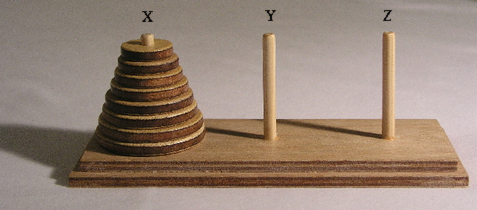
\includegraphics[width=180pt]{Tower-of-Hanoi.png}\\
\figcaption{Hanoi塔问题}\label{fig:hanoiTower}
\end{center}


现要求将X塔上的n个圆盘移动到Z上并仍按同样的顺序叠放,圆盘移动时必须遵循下列规则:
\begindot
\item 每次只能移动一个圆盘;
\item 圆盘可以插在X、Y和Z中的任一塔座上;
\item 任何时刻都不能将一个较大的圆盘压在较小的圆盘之上。
\myenddot
 
给出一个数$n$,求出最少步数的移动序列。


\subsubsection{输入}
一个整数 $n, n \leq 10$


\subsubsection{输出}
第一行一个整数$k$,表示最少的移动步数。

接下来$k$行,每行一句话,N from X to Y,表示把N号盘从X柱移动到Y柱。X,Y 属于\fn{\{'A','B','C'\}}


\subsubsection{样例输入}
\begin{Code}
3
\end{Code}


\subsubsection{样例输出}
\begin{Code}
7
1 from A to C
2 from A to B
1 from C to B
3 from A to C
1 from B to A
2 from B to C
1 from A to C
\end{Code}

\subsubsection{分析}
用递归。


\subsubsection{代码}

\begin{Codex}[label=hanoi.c]
#include <stdio.h>

/*
 * @brief 将塔座x上按直径有小到大且自上而下编号
 * 为1至n的n个圆盘按规则搬到塔座z上,y可用做辅助塔座.
 * @param[in] n 圆盘个数
 * @param[in] x 源塔座
 * @param[in] y 辅助塔座
 * @param[in] z 目标塔座
 * @return 无
 */
void hanoi(int n, char x, char y, char z) {
    if(n ==  1) {
        /* 将编号为n的圆盘从x移到z */
        printf("%d from %c to %c\n", n, x, z);
        return;
    } else {
        /* 将x上编号1至n-1的圆盘移到y,z作辅助塔 */
        hanoi(n-1, x, z, y);
        /* 将编号为n的圆盘从x移到z */
        printf("%d from %c to %c\n", n, x, z);
        /* 将y上编号1至n-1的圆盘移到z,x作辅助塔 */
        hanoi(n-1, y, x, z);
    }
}

int main() {
    int n;
    scanf("%d", &n);
    printf("%d\n", (1 << n) - 1); /* 总次数 */
    hanoi(n, 'A', 'B', 'C');
    return 0;
}
\end{Codex}


\subsubsection{相关的题目}
与本题相同的题目:
\begindot
\item wikioi 3145 汉诺塔游戏 , \myurl{http://www.wikioi.com/problem/3145/}
\myenddot

与本题相似的题目:
\begindot
\item  无
\myenddot


\subsection{进制转换}
\begin{Codex}[label=convert_base.cpp]
#include <stack>
#include <stdio.h>

 /**
  * @brief 进制转换,将一个10进制整数转化为 d进制,d<=16.
  * @param[in] n 整数n
  * @param[in] d d进制
  * @return 无
  */
void convert_base(int n, const int d) {
    std::stack<int> s;
    int e;

    while(n != 0) {
        e = n % d;
        s.push(e);
        n /= d;
    }
    while(!s.empty()) {
        e = s.top();
        s.pop();
        printf("%X", e);
    }
    return;
}

#define MAX 64 // 栈的最大长度
int stack[MAX];
int top = -1;
/**
 * @brief 进制转换,将一个10进制整数转化为 d进制,d<=16,更优化的版本.
 *
 * 如果可以预估栈的最大空间,则用数组来模拟栈,这时常用的一个技巧。
 * 这里,栈的最大长度是多少?假设CPU是64位,最大的整数则是2^64,由于
 * 数制最小为2,在这个进制下,数的位数最长,这就是栈的最大长度,最长为64。
 *
 * @param[in] n 整数n
 * @param[in] d d进制
 * @return 无
 */
void convert_base2(int n, const int d) {
    int e;

    while(n != 0) {
        e = n % d;
        stack[++top] = e; // push
        n /= d;
    }
    while(top >= 0) {
        e = stack[top--]; // pop
        printf("%X", e);
    }
    return;
}


/**
 * @brief 进制转换,将一个d进制整数转化为10进制,d<=16.
 * @param[in] s d进制整数
 * @param[in] d d进制
 * @return 10进制整数
 */
int restore(const char s[MAX], const int d) {
    int i;
    int result = 0;
    int one;

    for (i = 0; s[i] != '\0'; i++) {
        if (s[i] >= '0' && s[i] <= '9') one = s[i] - '0';
        else if (s[i] >= 'A' && s[i] <= 'F') one = s[i] - 'A' + 10;
        else one = s[i] - 'a' + 10; /* (s[i] >= 'a' && s[i] <= 'f') */
        
        result = result * d + one;
    }
    return result;
}
\end{Codex}

\section{队列} %%%%%%%%%%%%%%%%%%%%%%%%%%%%%%

\subsection{队列的C语言实现}
C++可以直接使用\fn{std::queue}。

\begin{Codex}[label=queue.c]
/** @file queue.c
  * @brief 队列,顺序存储,循环队列.
  * @author soulmachine@gmail.com
  */
#include <stdlib.h> /* for malloc(), free() */
#include <string.h> /* for memcpy() */

#ifndef __cplusplus
typedef char bool;
#define false 0
#define true 1
#endif

typedef int queue_elem_t; // 元素的类型

/*
  *@struct
  *@brief 队列的结构体定义.
  *@note 无
  */
typedef struct queue_t {
    int front;   /* 队头*/
    int rear;    /* 队尾*/
    int capacity; /* 容量大小,以元素为单位*/
    queue_elem_t *elems; /* 存放数据的内存块*/
}queue_t;

/**
  * @brief 创建队列.
  * @param[in] capacity 初始容量
  * @return 队列
  */
queue_t* queue_create(int capacity) {
    queue_t *q = (queue_t*)malloc(sizeof(queue_t));
    q->front = 0;
    q->rear = 0;
    q->capacity = capacity;
    q->elems = (queue_elem_t*)malloc(capacity * sizeof(queue_elem_t));
    return q;
}

/**
  * @brief 销毁队列.
  * @param[in] q 队列对象的指针
  * @return 无
  */
void queue_destroy(queue_t *q) {
    free(q->elems);
    free(q);
}

/**
  * @brief 判断队列是否为空.
  * @param[in] q 队列结构体的指针
  * @return 是空,返回TRUE,否则返回FALSE
  */
bool queue_empty(const queue_t *q) {
    return q->front == q->rear;
}

/**
 * @brief 获取元素个数.
 * @param[in] s 栈对象的指针
 * @return 元素个数
 */
int queue_size(const queue_t *q) {
    return (q->rear - q->front + q->capacity) % q->capacity;
}

/**
  * @brief 在队尾添加元素.
  * @param[in] q 指向队列结构体的指针
  * @param[in] x 要添加的元素
  * @return 无
  */
void queue_push(queue_t *q, const queue_elem_t x) {
    if( (q->rear+1) % q->capacity == q->front) { // 已满,重新分配内存
        queue_elem_t* tmp = (queue_elem_t*)malloc(
            q->capacity * 2 * sizeof(queue_elem_t));
        if(q->front < q->rear) {
            memcpy(tmp, q->elems + q->front,
                (q->rear - q->front) * sizeof(queue_elem_t));
            q->rear -= q->front;
            q->front = 0;
        } else if(q->front > q->rear) {
            /* 拷贝q->front 到q->capacity 之间的数据*/
            memcpy(tmp, q->elems + q->front,
                (q->capacity - q->front) * sizeof(queue_elem_t));
            /* 拷贝q->data[0] 到q->data[rear] 之间的数据*/
            memcpy(tmp +
                (q->capacity - q->front),
                q->elems, q->rear * sizeof(queue_elem_t));
            q->rear += q->capacity - q->front;
            q->front = 0;
        }
        free(q->elems);
        q->elems = tmp;
        q->capacity *= 2;
    }
    q->elems[q->rear] = x;
    q->rear = (q->rear + 1) % q->capacity;
}

/**
  * @brief 在队头删除元素.
  * @param[in] q 队列结构体的指针
  * @param[out] x 存放退出队列的元素
  * @return 无
  */
void queue_pop(queue_t *q) {
    q->front = (q->front + 1) % q->capacity;
}

/**
 * @brief 获取队首元素.
 * @param[in] q 队列对象的指针
 * @return 队首元素
 */
queue_elem_t queue_front(const queue_t *q) {
    return q->elems[q->front];
}

/**
 * @brief 获取队尾元素.
 * @param[in] q 队列对象的指针
 * @return 队尾元素
 */
queue_elem_t queue_back(const queue_t *q) {
    return q->elems[q->rear - 1];
}
\end{Codex}

\subsection{打印杨辉三角}

\begin{Codex}[label=yanghui_triangle.cpp]
#include <queue>
/**
 * @brief 打印杨辉三角系数.
 *
 * 分行打印二项式(a+b)^n展开式的系数。在输出上一行
 * 系数的同时,将其下一行的系数预先计算好,放入队列中。
 * 在各行系数之间插入一个0。
 *
 * @param[in] n (a+b)^n
 * @return 无
 */
void yanghui_triangle(const int n) {
    int i = 1;
    std::queue<int> q;
    /* 预先放入第一行的1 */
    q.push(i);

    for(i = 0; i <= n; i++) {     /* 逐行处理*/
        int j;
        int s = 0;
        q.push(s);      /* 在各行间插入一个0*/

        /* 处理第i行的i+2个系数(包括一个0)*/
        for(j = 0; j < i+2; j++) {
            int t;
            int tmp;
            t = q.front();  /*读取一个系数,放入t*/
            q.pop();
            tmp = s + t;      /* 计算下一行系数,并进队列*/
            q.push(tmp);
            s = t;            /* 打印一个系数,第i+2个是0*/
            if(j != i+1) {
                printf("%d ",s);    
            }
        }
        printf("\n"); 
    }
}
\end{Codex}
